\section{Wstęp teoretyczny}

\subsection{Procesor graficzny}
Procesory graficzne są specjalnym rodzajem procesorów,
pierwotnie stworzonych do akceleracji obliczeń graficznych.
Obliczenia te charakteryzują się dużą liczbą względnie prostych, podobnych operacji,
które mogą być przeprowadzone równolegle.
Taki model obliczeń nosi nazwę SIMD (Single Instruction Multiple Data)
i oznacza równoległe wykonywanie tej samej operacji dla wielu różnych danych wejściowych.
\par
Współczesne karty graficzne są zaprojektowanie do wykorzystania
ich możliwości równoległych obliczeń w znacznie szerszym obszarze niż
pierwotny cel akceleracji grafiki komputerowej.
Technologie \textit{OpenCL} oraz \textit{CUDA} umożliwiają
programowanie GPGPU -\textit{general purpose GPU} w 
dziedzinach takich jak obliczenia naukowe, machine learning oraz kryptografia.
\par
W mojej pracy, w celu przeprowadzenia ataku na krzywą eliptyczną, wykorzystałem
algorytm \textit{Rho Pollard'a}, który z niewielkimi modyfikacjami można bardzo skutecznie wykonywać
równolegle. Z tego powodu wykorzystanie GPU do kryptoanalizy, pozwala znacznie przyśpieszyć czas
obliczeń. W celu stworzenia programu na GPU wykorzystałem technologię Nvidia CUDA, głównie ze względu
na znacznie lepiej rozwinięty ekosystem oraz dostępność materiałów w internecie.
Standard OpenCL w przeciwieństwie do CUDA, jest \textit{open-source} oraz może zostać wykorzystany do programowania
kart graficznych innych producentów. Niestety jest zauważalnie
gorzej wspierany w przypadku kart graficznych Nvidia.
\par
\subsubsection{Model programowania CUDA}
Program napisany w CUDA, składa się z jednego lub więcej \textit{kernel'a} - funkcji programu,
która będzie się wykonywać równolegle na GPU, na każdym z uruchomionych wątków.
Wątki są grupowane w \textit{bloki}, które mogą się składać z 1 do 1024 wątków w przypadku \textit{CUDA 7.5} \cite{CudaDeveloper}.
Następnie bloki są uruchamiane na dostępnych \b{SM} - \textit{streaming multiprocessor}.
Karty graficzne Nvidia składają się zazwyczaj z kilkunastu SM, które mogą równocześnie uruchomić wiele
bloków, co pozwala na równoczesne wykonywanie kilkuset wątków.
Wątki w ramach jednego bloku dzielą pamięć współdzieloną \textit{shared memory} oraz wykonują się równocześnie.
Możliwe jest uruchomienie znacznie większej ilości bloków, niż może się jednocześnie wykonywać na dostępnych SM.
W takiej sytuacji niektóre bloki będą oczekiwać na wolne zasoby aż poprzednie nie zakończą pracy.
Dodatkowo, wątki w ramach bloku wykonują tą samą instrukcję w grupach po 32,
nazywanych \textit{warp'ami}.
W przypadku architektury SIMD ważne jest unikanie długich segmentów
warunkowych, ponieważ skutkuje to sekwencyjnymi obliczeniami.
W sytuacji gdy następuje rozgałęzienie kodu - \textit{branching},
część wątków w warp'ie musi czekać na pozostałe, skutkując sekwencyjnym wykonywaniem kodu.
Jest to szczególnie istotne dla wydajności działania programu na GPU.
\subsubsection{Hierarchia pamięci}
Kolejnym ważnym elementem który mocno wpływa na wydajność
programu, jest odpowiedni dostęp do pamięci.
Tak samo jak w zwykłym procesorze, GPU ma kilka warstw
pamięci które różnią się rozmiarem oraz czasem dostępu.
W CUDA można wyróżnić 3 najważniejsze warstwy pamięci:
\begin{itemize}
    \item Rejestry - najszybszy rodzaj pamięci, dostępny w ramach pojedynczego wątku.
    Ilość rejestrów dla każdego wątku jest jednak mocno ograniczona w przypadku
    uruchomienia wielu wątków równocześnie. Jeżeli program używa wiecej rejestrów niż jest dostępne,
    może wystąpić \textit{register spilling}, który wprowadza znaczne opóźnienia.
    \item \textit{Shared memory} - szybka pamięć współdzielona, która jest wspólna dla wątków w danym bloku. Jest ona ograniczona
    przez ilość pamięci w SM, na karcie graficznej z CUDA 7.5 jej rozmiar wynosi 64 KB \cite{CudaDeveloper}.
    Stosowana jest w przypadku, gdy wiele wątków musi się ze sobą komunikować lub w celu cache'owania danych
    i ograniczenia dostępu do znacznie wolniejszej pamięci globalnej.
    Zbyt duży rozmiar wykorzystywanej pamięci współdzielonej ogranicza ilość bloków które mogą jednocześnie się
    wykonywać na jednym SM.
    \item \textit{Global memory} - pamięć globalna DRAM, najwolniejsza oraz największa ze wszystkich warstw. Wykorzystywana głównie w celu
    komunikacji karty graficznej z procesorem, w celu przesyłania danych do obliczeń oraz zapisu wyników.
\end{itemize}
Dostępne są również dodatkowe rodzaje takie jak \textit{texture memory} oraz \textit{constant memory},
które różnią się optymalnym sposobem dostępu, jednak nie są wykorzystywane w tej pracy.

\subsection{Krzywe eliptyczne}
Zakładając, że ciało $\mathbb{K}$ ma charakterystykę różną od 2 i 3,
oraz że stałe $a, b \in \mathbb{K}$ spełniają warunek:
\[4a^3 + 27b^2 \neq 0\]
nieosobliwą krzywą eliptyczną nad ciałem $\mathbb{K}$ definiuje się jako zbiór punktów $(x,y) \in \mathbb{K} \times \mathbb{K}$,
spełniających równanie:
\[y^2 = x^3 + ax + b\]
wraz ze specjalnym punktem w nieskończoności $\mathcal{O}$, który pełni rolę elementu neutralnego
w działaniach grupowych
\cite{Stinson2021}.
\begin{figure}[H]
    \centering 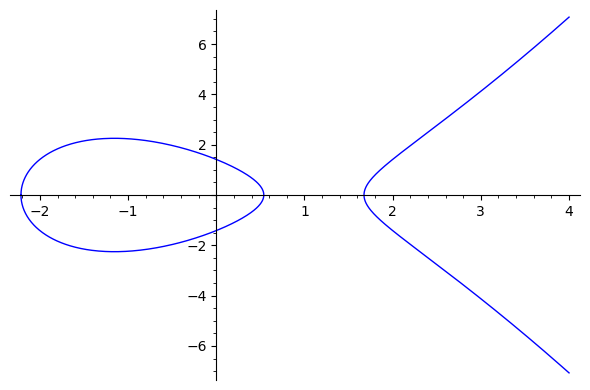
\includegraphics[width=0.8\linewidth]{sage/krzywa_-4_2.png}
    \caption{Krzywa eliptyczna $y^2=x^3-4+2$ nad ciałem liczb rzeczywistych}
\end{figure}

Krzywe eliptyczne zdefiniowane na liczbach rzeczywistych nie są kluczowe w
systemach kryptograficznych \cite*{Stinson2021}, ale takie ustawienia
pozwalają na prostsze przedstawienie niektórych zagadnień
np. dodawnie punktów na krzywej.


\subsubsection{Dodawanie punktów na krzywej eliptycznej}
Odpowiednie zdefiniowanie operacji dodawania punktów na krzywej eliptycznej
pozwala otrzymać grupę abelowa, złożoną z punktów krzywej oraz punktu w nieskończoności jako
elementu neutralnego.
\newline
\indent
Geometrycznie, dodawanie punktów na krzywej eliptycznej nad ciałem liczb rzeczywistych można przedstawić
jako połączenie dwóch punktów $P$ i $Q$ prostopadłą linią, która przecina krzywą w trzecim
punkcie, $R'$. Następnie, wynikowy punkt $R$, będący sumą $P+QP+Q$, znajdujemy przez
odbicie punktu $R'$ względem osi $x$. W przypadku podwojenia punktu, czyli dodawania
punktu P do siebie samego, rysujemy styczną do krzywej w punkcie $P$, która przecina
krzywą w nowym punkcie. Odbicie tego punktu względem osi $x$ daje nam wynik $2P$ \cite{Chrzeszczyk2010}\cite{Stinson2021}.
\begin{figure}[!h]
    \centering 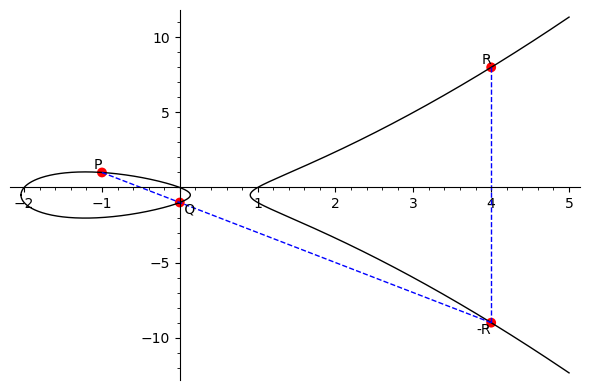
\includegraphics[width=0.8\linewidth]{sage/elliptic_rational_point_addition.png}
    \caption{P + Q na krzywej eliptycznej $y^2+y=x^3-x^2+2x$}
\end{figure}
\par
Definując dodawanie punktów na krzywej eliptycznej w sposób algebraiczny otrzymujemy następujące wzory:
\begin{enumerate}
    \item Przypadek, gdy \( P \neq Q \):
          \begin{align}
              \lambda & = \frac{y_2 - y_1}{x_2 - x_1}, \\
              x_3     & = \lambda^2 - x_1 - x_2,       \\
              y_3     & = \lambda(x_1 - x_3) - y_1
          \end{align}
    \item Przypadek, gdy \( P = Q \):
          \begin{align*}
              \lambda & = \frac{3x_1^2 + a}{2y_1}, \\
              x_3     & = \lambda^2 - 2x_1,        \\
              y_3     & = \lambda(x_1 - x_3) - y_1
          \end{align*}
    \item Szczególny przypadek, gdy \( P = -Q \):
          \begin{align*}
              P + (-P) = \mathcal{O}
          \end{align*}
\end{enumerate}
Dodatkowo odwrotność punktu na krzywej $P$ definujemy jako $-P = (x, -y)$ \cite{Stinson2021}.


\subsubsection{Krzywe eliptyczne na ciele skończonym}
Krzywe eliptyczne zdefiniowane na ciele skończonym $F_p$ oraz $F_{p^n}$ mają kluczowe znaczenie w kryptografii.
W swojej pracy skupiłem się wyłącznie na krzywych zdefiniowanych na ciele skończonym $F_p$ gdzie $p$ jest liczbą pierwszą.
\par
Wykres krzywej eliptycznej nad ciałem $F_p$ nie przypomina krzywej zdefiniowanej na liczbach rzeczywistych.
Krzywa taka składa się z dyskretnych punktów, których współrzędne należą do ciała
na którym jest opisana.
Operacje na krzywej nad ciałem skończonym są zdefiniowane
za pomocą tych samych wzorów algebraicznych, co w przypadku ciała liczb rzeczywistych,
jednak wszystkie działania są wykonywane na ciele $F_p$.
\begin{figure}[!h]
    \centering 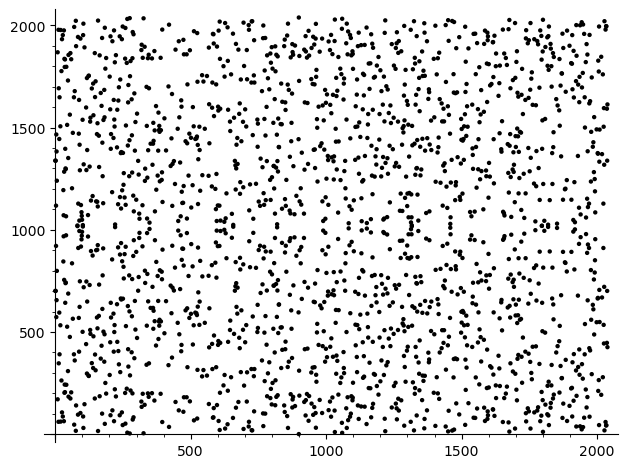
\includegraphics[width=0.8\linewidth]{sage/ec_2_11-9.png}
    \caption{Krzywa eliptyczna $y^2=x^3-4+2$ nad $GF(2^{11} - 9)$}
\end{figure}


\subsubsection{Problem logarytmu dyskretnego}
Problem logarytmu dyskretnego (\textbf{DLP}) jest
podstawą kryptosystemów oparych o grupy.
Jednymi z bardziej znanych są kryptosystem ElGamala oraz protokół wymiany
kluczy Diffie-Hellmana'a.
\\ Problem logarytmu dyskretnego można zdefiniować na grupach cyklicznych.
zarówno na grupie multiplikatywnej $(\mathbb{G},\cdot)$
oraz grupie addytywnej $(\mathbb{G}, +)$, przy odpowiednim zdefiniowaniu działań grupowych.

Jeżeli G jest grupą cykliczną a $\gamma$ jej generatorem, to logarytmem dyskretnym
elementu $\alpha \in G$ nazywamy najmniejszą nieujemną liczbę całkowitą $x$ taką, że:
\[x = \log_{\gamma}{\alpha}\]

Uważa się, że problem logarytmu dyskretnego jest trudny, ponieważ nie istnieje
algorytm, który znajduje $x$ w czasie wielomianowym\cite{Stinson2021}.


\subsubsection{Problem logarytmu dyskretnego na krzywej eliptycznej}
W przypadku krypografii opartej o krzywe eliptyczne, DLP dotyczy cykliczej
grupy addytywnej $(\mathbb{E},+)$ zdefiniowanej na krzywej eliptycznej.
Aby utworzyć taką grupę, wybieramy punkt $P$ na krzywej eliptycznej $\mathbb{E}$,
który będzie generatorem grupy. Wtedy grupa addytywna $\mathbb{E}$ jest generowana przez
kolejne \textit{potęgi} punktu $P$:
\[\ \langle P \rangle = \{P, 2P, 3P, \ldots, nP = \mathcal{O}\}\]
W takim przypadku, ponieważ operacją na grupie jest dodawanie modulo n, to działanie
potęgowania przedstawia się jako zwielokrotnienie punktu $P$:
\[x \cdot P = Q \textrm{ (mod } n)\]
Analogicznie do problemu logarytmu dyskretnego na grupach multiplikatywnych,
problem logarytmu dyskretnego na krzywej eliptycznej polega na znalezieniu
$x$.
\par
Przy odpowiednim wyborze grupy addytywnej, rozwiązanie problemu logarytmu dyskretnego,
tj. znalezienie $x$,
jest trudne \cite{Stinson2021}.


\subsection{Algorytm Rho Pollarda}
 
RYSUNEK LITERKI RHO (bo jak inaczej bez tego mówic o rho pollardzie :))

DODAC OPIS, co się dzieje po znalezieniu kolizji, jak to pozwala obliczyć logarytm dyskretny

CZY TRZEBA opisywać algorym sekwencyjny skoro i tak korzystam z równoległego? Moze samo odesłanie do literatury
\par
DO UZUPEŁNIENIA
\par
\par
Najszybszym znanym algorytmem rozwiązującym problem logarytmu dyskretnego na krzywej eliptycznej
jest algorytm Rho Pollarda,
zaproponowany przez Johna Pollarda w 1978 roku \cite{Pollard1978}.
Pozwala on na znalezienie logarytmu dyskretnego w czasie $O(\sqrt{n})$,
jednak jest to jedynie czas \textit{oczekiwany}, ponieważ ze względu na losową naturę algorytmu \cite{Blake2005}.
W porównaniu do innego znanego algorytmu, Baby-Step Giant-Step \cite{Stinson2021}, algorytm Rho Pollarda jest bardziej
efektywny pamięciowo, nie wymagając
przestrzeni $O(\sqrt{n})$ a jedynie $O(1)$ w wersji sekwencyjnej \cite{Stinson2021}\cite{Blake2005}.
\par
Klasyczny algorytm Rho Pollarda, oparty o poszukiwanie cyklu, słabo się skaluje w przypadku zrównoleglenia,
osiągając jedynie przyśpieszenie rzędu $O(\sqrt{m})$ dla $m$ procesorów \cite{Goldberg}.
Dlatego w swojej pracy wykorzystałem równoległą wersję algorytmu, zaproponowaną przez Van Oorschota i Wienera \cite{Oorschot}.
% \par
% Idea klasycznego algorytmu Rho Pollarda, polega na poszukiwaniu kolizji punktów:
% $$
% X_i = X_{2i}
% $$
% takich, że:
% $$
% X_i = a_i \cdot P + b_i \cdot Q
% $$
% $$
% X_{2i} = a_{2i} \cdot P + b_{2i} \cdot Q
% $$
% Jeżeli znajdziemy kolizję punktów $X_i$ i $X_j$,
% to za pomocą odpowiednich przekształceń możemy obliczyć logarytm dyskretny $x$:
% $$
% a_i \cdot P + b_i \cdot Q = a_j \cdot P + b_j \cdot Q
% $$
% $$
% (a_i - a_j) \cdot P = (b_j - b_i) \cdot Q
% $$
% $$
% x = \frac{b_j - b_i}{a_i - a_j}
% $$

% Zakładając, że $P$ jest generatorem grupy na krzywej eliptycznej, oraz, że chcemy obliczyć logaryytm dyskretny $x$:
% $$
% x\cdot P = Q
% $$
% Idea algorytmu polega na iteracyjnym stosowaniu losowo wyglądającej funkcji $f$, która generuje kolejne trójki
% w postaci $(X_i, a_i, b_i)$, gdzie $X_i$ jest punktem na krzywej eliptycznej, a $a_i$ oraz $b_i$ są liczbami całkowitymi:
% \[
%     f(X, a, b) =
%     \begin{cases}
%         (X + Q,a, b + 1)               & \text{jeśli } X \in S_1, \\
%         (2X, 2a, 2b) & \text{jeśli } X \in S_2, \\
%         (X + P, a+1, b)                           & \text{jeśli } X \in S_3,
%     \end{cases}
% \]

\subsubsection{Równoległy algorytm Rho Pollarda}
Równoległa wersja algorytmu Rho Pollarda, zakłada zastosowanie wielu równoległych ścieżek błądzenia.
\par
Jednostki obliczeniowe poszukują wtedy specalnych punktów nazywanych wyróźnionymi,
które następnie są przekazywane do centralnego serwera w celu znalezienia kolizji między nimi.
\par
Ponieważ sprawdzenie, czy punkt jest wyróźniony następuje w każdej iteracji,
ważne jest aby kryterium decydujące o uznaniu punktu za wyróźniony, było możliwie
szybkie do sprawdzenia.
Często stosowaną metodą, jest sprawdzanie ilości zer na początku lub na końcu binarnej reprezentacji współrzędnej $x$.
\par
Adding walk zakłada jedynie wykonywanie kolejnych operacji dodawania punktów.

Niech $W_0$ będzie punktem startowym, a $f$ funkcją haszującą $f: \langle P \rangle \rightarrow \{1,..s\}$ o możliwie jednostajnym rozkładzie.
Następnie, potrzebujemy tablicy wstępnie obliczonych punktów:
$R_i = c_i P + d_i Q$ dla $0 \leq i \leq s - 1$.
Funkcja iteracyjna jest wtedy zdefiniowana w następujący sposób:
$$
    W_{i+1} = W_i + R_{f(W_i)}
$$
Ważną kwestią jest też rozmiar tablicy z punktami wstepnie obliczonymi.
Zbyt mały rozmiar powoduje, że funkcja nie będzie dostatecznie losowa.
W eksperymentach praktycznych pokazano, że dla $s \geq 16$, funkcja zapewnia
wystarczający poziom losowości,  niezależnie od rozmiaru grupy.
 \cite{Teske2000}
\par
Istotną zaletą tej funkcji w przypadku programu uruchamianego na GPU,
jest uniknięcie rozgałęzień podczas każdej iteracji, co jest szczególnie istotne w przypadku architektury SIMD.
Prawie zawsze wykonujemy tą samą operację dodawania dwóch punktów,
poza mało prawdopodobnym przypadkiem w którym $W_i == R_{f(W_i)}$.
\par
\newpage